\section{$OR$, Dirac Notation}

\subsection*{Classical Query complexity of $OR$}
\begin{propbox}{}
    $D(OR_n) = n$.
\end{propbox}

\begin{proof}
    $n \geq D(OR_n)$ is obvious (in fact is obvious for any function on $n$-bits that $n$ is an upper bound). Since $D(f)$ is a minimum over decision trees computing $f$, simply take the tree which checks every bit in the input, outputting $1$ if any of the bits are $1$, and outputting $0$ if all of the bits are $0$ (the worst case/depth of the tree is checking all of the bits and finding all are zero).

    $n \leq D(OR_n)$ is not quite as simple. We develop an ``adversary argument'' for this purpose. 

    In general, we imagine a two-player game between the Algorithm and an Adversary based on a Boolean function $f$. The game is played as follows:
    \begin{enumerate}
        \item The Adversary maintains a bag of strings $S$ containing the domain, usually $\set{0, 1}^n$.
        \item At each round, the Algorithm is allowed to query a new bit, say, the $i$th, and te Adversary answers wit $x_i \in \set{y_i, \exists y \in S}$, i.e. the Adversary chooses an output that describes an element in $S$. The set $S$ is updated to remove all $y$ such that $y_i \neq x_i$.
        \item The game ends if $f(y)$ takes the same value for all $y \in S$
    \end{enumerate}
    The length of any such game is a lower bound on $D(f)$. Informally - if we fix a decision tree for $f$, the Algorithm in the game asks the Adversaries queries following the decision tree, using the responses to navigate down the tree. $S$ corresponds to all strings that would have lead the algorithm to the current node, and the game ends if all leaf nodes under the current node have the same level (because the Algorithm can output the value of $f$ and does not need to query any new bits).The game proceeding to $k$ rounds therefore implies the depth of the decision tree is at least $k$.

    Having discussed the technique, we describe the procedure for $OR_n$. Fix an algorithm/decision tree. Consider the adversary that returns every query with $0$. After any $n - 1$ queries, there is some index $i \in [n]$ not queried yet (suppose WLOG $i = 1$). At this point, the Adversary's bag contains at least 2 strings evaluating to different values, namely $0^n$ and $10^{n-1}$. Thus, the game proceeds to the $n$th round, giving $D(OR_n) \geq n$.
\end{proof}

\begin{propbox}{}
    $R_{\e}(OR_n) \geq (1-2\e)n$
\end{propbox}
\begin{proof}
    Suppose $\exists$ RDT $\tau$ of depth $k \in \set{1, 2, \ldots, n}$ that computes $OR_n$ with bounded error $\e$. Then, $\forall x \in \set{0, 1}^n$, we have:
    \begin{equation}
        Pr^T_{T \leftarrow \tau}[T(x) = OR_n(x)] \geq 1-\e
    \end{equation}
    Then the LHS is equivalent to:
    \begin{equation}
        \sum_{TDDT}\mathbb{1}[T(x) = OR_n(x)] Pr[T \leftarrow \tau] \geq 1 - \e
    \end{equation}
    Consider a probability distribution on $\set{0, 1}^n$, then take $\mathbb{E}_{x \leftarrow \mu}[(*)]$. Using the linearity of expectation and hitting the indicator function with the expectyation, we get:
    \begin{equation}\label{eq-lec2proof2}
        \sum_{TDDT}Pr_{x \leftarrow \mu}[T(x) = OR_n(x)]Pr[T \leftarrow \tau] \geq 1 - \e
    \end{equation}
    Now, there exists $T^*$ a DDT such that:
    \begin{equation}
        Pr_{x \leftarrow \mu}[T^*(x) = OR_n(x)] \geq 1 - \e
    \end{equation}
    There are many ways to see this. One way; suppose for every $T^*$ did not hold. Then, the $Pr_{x \leftarrow \mu}[T(x) = OR_n(x)]$ is less than $1 - \e$, which violates the equality in Eq. \eqref{eq-lec2proof2} because $Pr[T \leftarrow \tau] < 1$ (And sums to one taken over the entire $TDDT$). This is a fairly standard technique when proving bounds with randomized algorithms.
    
    Now, lets define $\mu$ as follows:
    \begin{equation}
        \mu(x) = \begin{cases}
            \frac{1}{2n} & \text{if $x$ is of Hamming weight 1.}
            \\ \frac{1}{2} & \text{if } x = 0^n
            \\ 0 & \text{otherwise}
        \end{cases}
    \end{equation}
    Note the Hamming weight is just the number of ones in the bit string, i.e. for $x \in \set{0, 1}^n$ we have $\abs{x} = \sum_{i=1}^n x_i$. 

    Suppose that when the decision tree sees all zeroes, i.e. $x$ is the all zero string, it does the reasonable thing and outputs $0$ (Checking the other case where it outputs 1 will be your homework!). This has probability $Pr_{x \leftarrow \mu}[T^*(x) = OR_n(x)] = \frac{1}{2} \cdot 1 = \frac{1}{2}$. Next, how many bit strings are of Hamming weight 1 such that its $i_1 \ldots i_{k}$ are all zero. This happens to be $k$ bit strings ($i_{k+1}$ to $i_n$ could be $1$). So we have $n-k$ paths where the DDT spits out the wrong thing (i.e. spits out 0) while the $OR_n$ is 1, and $k$ where it gives the correct answer. The probability of a Hamming weight 1 bitstring is $\frac{1}{2n}$.  So, we get:
    \begin{equation}
        Pr_{x \leftarrow \mu}[T^*(x) = OR_n(x)] = \frac{1}{2} \cdot 1 + \frac{k}{2n} \geq 1 - \e
    \end{equation}
    Then:
    \begin{equation}
        \frac{k}{2n} \geq \frac{1}{2} - \e \implies k \geq (1-2\e)n
    \end{equation}
    which proves the claim.
\end{proof}


\begin{figure}[htbp!]
    \centering
    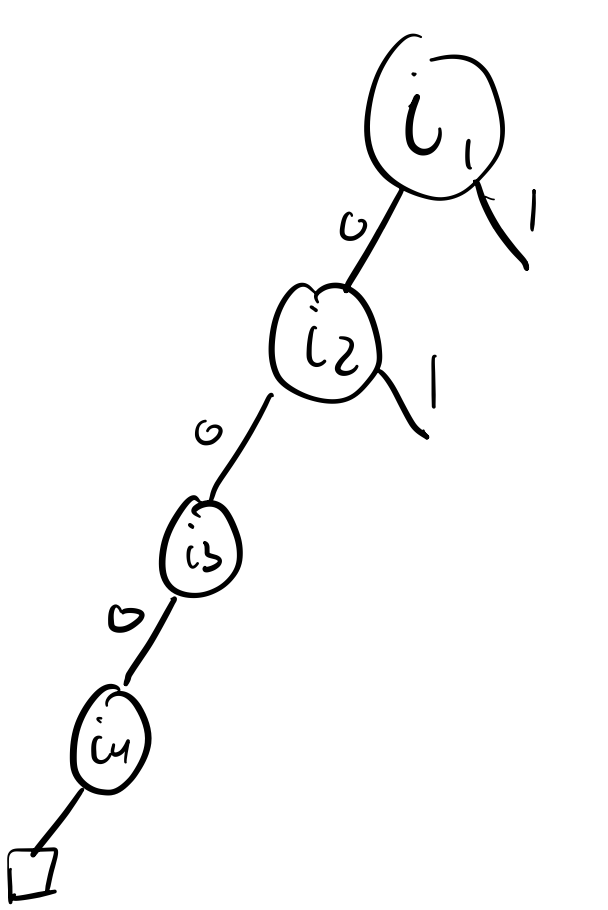
\includegraphics[scale=0.8]{Images/fig-lec2-orn.png}
    \caption{Visualization of above argument}
    \label{lec2-orn}
\end{figure}

Two notes:
\begin{enumerate}
    \item This seemingly magical approach where we fix a decision tree and then choosing a distribution usually works for proving lower bounds. The answer actually turns out to be yes.  The steps at the beginning of this proof can always be used to give the optimal lower bound on randomized query complexy - this is Yao's principle.
    \item The $OR_n: \set{0, 1}^n \to \set{0, 1}$ function has been considered. We can consider a restriction of the domain $OR_n^{0, 1}: \set{0^n} \cup \set{\text{Hamming weight} \vert \set{strings}} \to \set{0, 1}$ - note that $R_\e(OR_n^{0, 1}) \geq (1-2\e)n$ still holds.
\end{enumerate}

\subsection*{Dirac notation}
For $n \in \NN$, an $d$-dimensional quantum state is a unit vector $v \in \CC^d$, written as $\ket{v}$ (``ket $v$''), where unit refers to the vector having an $l2$-norm of $1$, i.e. $\sum_{i=1}^d \abs{v_i}^2 = 1$. 

We can then define $\bra{v}$ (``bra $v$'') as the complex conjugate transpose of $v$. 

$\braket{u}{v}$ is just the inner product of $u$ and $v$, $\braket{u}{v} = \sum_{i=1}^d u^*_i v_i = \langle u, v \rangle$. This is the ``bracket''!

We can also put things together as $\dyad{u}{v}$, which is a matrix/outer product:
\begin{equation}
    \dyad{v}{u} = \m{v_1 \\ v_2 \\ v_3}\m{u_1^* & u_2^* & u_3^*} = \m{v_1u_1^* & v_1u_2^* & v_1u_3^* \\ v_2u_1^* & v_2u_2^* & v_2u_3^* \\ v_3u_1^* & v_3u_2^* & v_3u_3^*}
\end{equation}

Given $\ket{v_1} \in \CC^{d_1}, \ket{v_2} \in \CC^{d_2}$, we denote $\ket{v_1}\ket{v_2} \coloneqq \ket{v_1} \otimes \ket{v_n} \in \CC^{d_1 \cdot d_2}$. This is known as the tensor, or Kronecker product. Explicitly:
\begin{equation}
    \ket{v} \otimes \ket{u} = \m{v_1 \\ v_2} \otimes \m{u_1 \\ u_2 \\ u_3} = \m{v_1u_1 \\ v_1 u_2 \\ v_1 u_3 \\ v_2 u_1 \\ v_2 u_2 \\ v_2 u_3}.
\end{equation}
The ``computational basis'' of $\CC^d$ is the basis (shown below for $d = 4$, but easily generalizes):
\begin{equation}
    \ket{0} = \m{1 \\ 0 \\ 0 \\ 0}, \ket{1} = \m{0 \\ 1 \\ 0 \\ 0}, \ket{2} = \m{0 \\ 0 \\ 1 \\ 0}, \ket{3} = \m{0 \\ 0 \\ 0 \\ 1}
\end{equation}
so $\ket{v} = \sum_{i=1}^d v_i \ket{i}$. 

An $n$-qubit quantum state $v$ is a vector in $\CC^{2n}$. Then, any such $\ket{v}$ can be expanded as follows:
\begin{equation}
    \ket{v} = \sum_{x \in \set{0, 1}^n}\alpha_x \ket{x_1}\ket{x_2}\ket{x_3}\ldots \ket{x_n}
\end{equation}
where $\alpha_x \in \CC$. E.g. for $n = 3$, we have:
\begin{equation}
    \ket{0}\ket{1}\ket{1} = \m{1 \\ 0} \otimes \m{0 \\ 1} \otimes \m{0 \\ 1} = \m{0\\0\\0\\1\\0\\0\\0\\0}
\end{equation}

We can also take tensor products of matrices:
\begin{equation}
    \m{u_{11} & u_{12} \\ u_{21} & u_{22}} \otimes V = \m{u_{11}V & u_{12}V \\ u_{21}V & u_{22}V}.
\end{equation}

\begin{defbox}{: Projective measurement}
    Let $\Gamma$ be an alphabet. An $\Gamma$-outcome projective measurement on $\CC^d$ is a set of $\abs{\Gamma}$ matrices $\Pi_1, \Pi_2, \ldots \Pi_{\abs{\Gamma}} \in \CC^{d \times d}$ such that the $\set{\Pi_i}_i$ are a set of orthogonal projectors, i.e. $\forall i, j$ we have $\Pi_i \Pi_j = \delta_{ij}\Pi_i$ and $\sum_{i=1}^{\abs{\Gamma}} \Pi_i = \II_d$.
\end{defbox}
\begin{defbox}{: Performing a measurement}
    Let $\mathcal{M}$ be a $\Gamma$-outcome projective measurement on $\CC^d$, i.e. $\mathcal{M} = \set{\Pi_1, \ldots, \Pi_{\abs{\Gamma}}}$ and let $\ket{\psi} \in \CC^d$. Then to measure $\mathcal{M}$ produces the following:
    \begin{enumerate}
        \item Output $i \in [\abs{\Gamma}]$ with probability:
        \begin{equation}
            p(i) = \norm{\Pi_i \ket{\psi}}^2 = \bra{\psi}\Pi_i \ket{\psi}
        \end{equation}
        \item The state becomes:
        \begin{equation}
            \ket{\psi} = \frac{\Pi_i \ket{\psi}}{\norm{\Pi_i \ket{\psi}}}
        \end{equation}
        where the denominator appears so it remains normalized.
    \end{enumerate}
\end{defbox}

\begin{defbox}{: Computational Basis measurement}
    The computational basis measurement on $\CC^d$ is defined by the following [$d$]-outcome measurement $\dyad{0}{0}, \dyad{1}{1}, \ldots \dyad{d-1}{d-1}$. 
\end{defbox}

\subsection*{An example of projecting into a subspace}
Consider the Hilbert space $\CC^2 \otimes \CC^2 \cong \CC^4$ of two qubits. Suppose we want to measure the first qubit, but not the second qubit. The projectors corresponding to this measurement are:
\begin{equation}
    \Pi_0 = \dyad{0}{0} \otimes \II_2, \quad \Pi_1 = \dyad{1}{1} \otimes \II_2. 
\end{equation}
which have the action of projecting the first qubit onto one of the two computational basis states, and doing nothing to the second qubit. We can verify that they obey the conditions for being a set of orthogonal projectors:
\begin{equation}
    \Pi_0^2 = (\dyad{0}{0})^2 \otimes (\II_2)^2 = \dyad{0}{0} \otimes \II_2 = \Pi_0
\end{equation}
\begin{equation}
    \Pi_1^2 = (\dyad{1}{1})^2 \otimes (\II_2)^2 = \dyad{1}{1} \otimes \II_2 = \Pi_1
\end{equation}
\begin{equation}
    \Pi_0 \Pi_1 = (\ket{0}\braket{0}{1}\bra{1}) \otimes \II_2 = 0
\end{equation}
\begin{equation}
    \Pi_0 + \Pi_1 = (\dyad{0}{0} + \dyad{1}{1}) \otimes \II_2 = \II_2 \otimes \II_2 = \II_4
\end{equation}
but notably, the number of projectors in the set is strictly less than the dimension of the underlying Hilbert space, i.e. this corresponds to a measurement of a subspace.

\subsection*{Quantum Query Algorithm}
\begin{defbox}{: Quantum query algorithm}
    A quantum query algorithm of depth $d \in \NN$ is specified by the following data:
    \begin{enumerate}
        \item $w \in \NN$
        \item $d + 1$ unitary matrices $U_0, U_1, \ldots U_d$ acting on $\CC^n \otimes \CC^m \otimes \CC^w$. 
        \item A $\Gamma$-outcome projective measurement on $\CC^{nmw}$. 
    \end{enumerate}
\end{defbox}

\begin{defbox}{: Quantum oracle}
    For $x \in \set{0, 1, \ldots, m-1}^n$, the ``quantum oracle'' of $x$ is the unitary matrix $O_x \in \CC^{nm \times nm}$ defined by $O_x\ket{i}\ket{j} = \ket{i}\ket{j + x_i \mod m}$, for all $i \in \set{0, \ldots, n -1 }$ and $j \in \set{0, 1, \ldots m - 1}$. 

    In particular, we often deal with the case where $m = 2$, where:
    \begin{equation}
        O_x\ket{i}\ket{b} = \ket{i}\ket{b \oplus x_i}
    \end{equation}
\end{defbox}
